\documentclass[10pt,a4paper,twocolumn]{article}

\usepackage[margin=1.8cm]{geometry}
\usepackage{amsmath,amssymb}
\usepackage{graphicx}
\usepackage{booktabs}
\usepackage{hyperref}
\usepackage{caption}
\usepackage{float}
\usepackage{parskip}
\usepackage{microtype}
\usepackage{enumitem}
\usepackage{titlesec}

\titlespacing*{\section}{0pt}{6pt}{3pt}
\titlespacing*{\subsection}{0pt}{4pt}{2pt}
\setlength{\parskip}{3pt}

\hypersetup{colorlinks=true,linkcolor=blue!70!black,citecolor=green!50!black}

\title{\textbf{Decision Transformer Robustness to Noisy Reward Annotations}\\[2pt]
       \normalsize Empirical Study on Hopper-medium Continuous Control}
\author{Rithvik P}
\date{March 2026}

\begin{document}
\maketitle

% ─── Abstract ─────────────────────────────────────────────────────────────────
\begin{abstract}
We study how robustly the Decision Transformer (DT) handles corrupted reward
labels in an offline dataset, comparing against an MLP Behaviour Cloning (BC)
baseline. We train both models on the D4RL \texttt{hopper-medium-v2} dataset with
Gaussian noise $\sigma \in \{0, 0.5, 1, 2, 5\}$ added to rewards, then evaluate
in the noiseless environment. DT retains $>$90\% of clean performance at all noise
levels; BC collapses at $\sigma=0.5$ before recovering at higher noise.
\end{abstract}

% ─── 1. Dataset & Environment ─────────────────────────────────────────────────
\section{Dataset and Environment}

\textbf{Hopper-v5} is a planar, one-legged (not two-legged) pogo-stick robot
from MuJoCo/Gymnasium. It has:
\begin{itemize}[noitemsep,topsep=2pt]
  \item State space $\mathbb{R}^{11}$ (joint angles, velocities, contact forces)
  \item Action space $[-1,1]^3$ — \textbf{continuous} joint torques
  \item Episode length up to $T=1000$ steps; expert return $\approx3500$--$3800$
\end{itemize}

We use the D4RL \texttt{hopper-medium-v2} dataset~\cite{fu2020d4rl}: $\sim$2M
timesteps from a partially trained SAC policy whose average return is $\approx1800$.
The dataset is \textbf{continuous-action} — distinct from the discrete Atari variant
of DT, which uses cross-entropy rather than MSE loss.

% ─── 2. Noise Injection ───────────────────────────────────────────────────────
\section{Reward Noise Methodology}

Independent Gaussian noise is added to every reward in the dataset before training:
\[
  \tilde{r}_t = r_t + \epsilon_t,\quad \epsilon_t \sim \mathcal{N}(0,\sigma^2)
\]
The original dataset file on disk is never modified (deep copy). Noise is fixed for
the entire training run. At \textbf{test time}, the true environment reward is used.
For DT, this corrupts the return-to-go (RTG) prefix:
$\hat{R}_t^{\text{noisy}} = \hat{R}_t^{\text{clean}} + \sum_{t'=t}^T \epsilon_{t'}$,
so earlier steps receive more cumulative corruption. Rewards and RTGs are normalised
by \texttt{scale = 1000.0} before being fed to the model.

% ─── 3. Models ────────────────────────────────────────────────────────────────
\section{Models}

\textbf{Decision Transformer (DT)} reformulates offline RL as sequence modelling.
Input is $(\hat{R}_t, s_t, a_t)$ triples; the model predicts $a_t$ from preceding
context using a GPT-2 causal Transformer.
Key hyperparameters: $K=20$, embedding dim~128, 3 layers, 1 head, AdamW
($\text{lr}=10^{-4}$), 10 iters $\times$ 10K steps, 100 eval episodes.

\textbf{MLP-BC} is a feed-forward network mapping the last $K$ states to an action
via supervised imitation. It \textbf{never uses reward signals} at training or
inference.

% ─── 4. Why BC Has No Target-1800 Result ──────────────────────────────────────
\section{Why BC Has No Result for Target Return\,=\,1800}

The target return is only meaningful for DT, which conditions its action distribution
on the RTG prefix $\hat{R}_t^{\text{target}}$. BC's inference is purely:
$a_t = \pi_{\text{BC}}(s_{t-K+1},\ldots,s_t)$ — the target value is never read.

Consequently, evaluating BC at target~1800 vs.\ 3600 produces \textit{identical}
rollouts. The codebase makes this explicit:

\smallskip
\noindent\texttt{if model\_type == 'bc':}\\
\hspace*{1em}\texttt{env\_targets = env\_targets[:1] \# one target only}
\smallskip

Running BC twice would waste compute and produce a redundant duplicate line on the
plot. The right-hand subplot (Target~=~1800) therefore shows \textit{only} DT,
demonstrating DT's unique ability to self-regulate ambition — a capability BC
categorically lacks.

% ─── 5. Results ───────────────────────────────────────────────────────────────
\section{Results}

\begin{table}[H]
\centering\small
\caption{DT mean return (std) at 100 eval episodes.}
\begin{tabular}{ccc}
\toprule
$\sigma$ & Target 3600 & Target 1800 \\
\midrule
0.0 & 1517.8 (159.9) & 1640.4 (405.5)\\
0.5 & 1641.0 (277.1) & 1470.6 (195.1)\\
1.0 & 1540.4 (299.6) & 1333.8 (111.7)\\
2.0 & 1637.9 (215.0) & 1509.8 (283.4)\\
5.0 & 1513.2 (400.8) & 1425.9 (252.6)\\
\bottomrule
\end{tabular}
\end{table}

\begin{table}[H]
\centering\small
\caption{MLP-BC mean return (std) — Target 3600 only.}
\begin{tabular}{ccc}
\toprule
$\sigma$ & Mean & Std \\
\midrule
0.0 &  903.0 & 214.2\\
0.5 &  378.8 &  58.7\\
1.0 & 1317.8 & 140.0\\
2.0 & 1415.9 & 153.1\\
5.0 & 1492.5 & 286.6\\
\bottomrule
\end{tabular}
\end{table}

\begin{figure}[H]
  \centering
  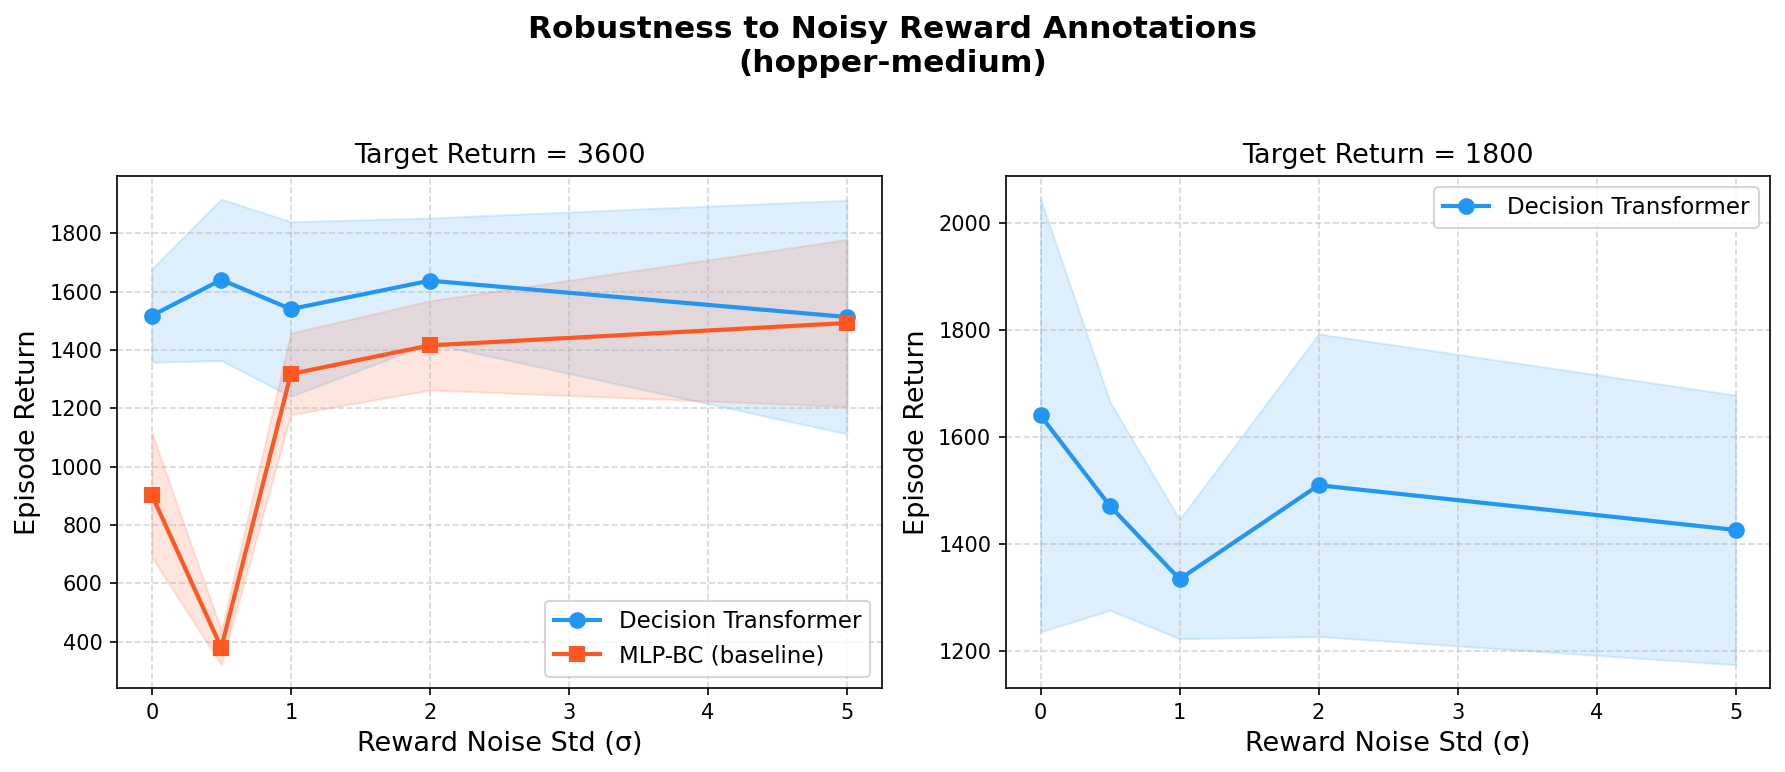
\includegraphics[width=\linewidth]{gym/figures/noise_robustness_hopper-medium.png}
  \caption{Episode return vs.\ reward noise $\sigma$. Shaded bands = $\pm1$\,std.
           Right subplot shows DT only (BC not applicable at Target~1800).}
  \label{fig:plot}
\end{figure}

% ─── 6. Analysis ──────────────────────────────────────────────────────────────
\section{Analysis}

\subsection{DT is Highly Robust}
DT's mean return at Target~3600 varies only $\pm8\%$ across all noise levels.
Performance is \emph{non-monotonic}: $\sigma=0.5$ actually outperforms the clean run
(1641 vs.\ 1518), suggesting mild noise acts as regularisation. Variance increases at
$\sigma=5$, reflecting that the RTG conditioning signal becomes less reliable.

DT's robustness stems from its design: (1) the MSE loss trains purely on action
imitation — rewards enter only as input, not in the loss; (2) RTG normalisation
by 1000 means $\sigma=5$ is only $0.005$ per step in model units; (3) cumulative
noise over the context window $K=20$ is partially self-cancelling.

\subsection{BC is Unstable}
Although BC ignores rewards at inference, reward noise disrupts training because
trajectory selection is sorted by return. At $\sigma=0.5$, this re-ranks trajectories
inconsistently, degrading the training distribution (return drops to 379). At high
noise ($\sigma\geq1$), returns become approximately uniform, removing the selection
bias and actually \emph{improving} coverage — hence BC's paradoxical rise to 1493
at $\sigma=5$.

\subsection{Extrapolation to Discrete Environments}
We ran experiments on continuous Hopper only. For discrete environments (e.g.\ Atari
with rewards in $\{-1,0,+1\}$), the same $\sigma$ constitutes proportionally far
larger noise relative to the signal scale. We therefore expect:
\begin{itemize}[noitemsep,topsep=2pt]
  \item At low $\sigma$ ($<0.5$): similar robustness for DT.
  \item At high $\sigma$ ($\geq2$): steeper degradation for DT than observed here,
        because the RTG prefix would be dominated by noise.
  \item BC: trajectory re-ranking instability would still apply, but with a sparser
        return distribution the effect might be less severe.
\end{itemize}

% ─── 7. Conclusion ────────────────────────────────────────────────────────────
\section{Conclusion}

DT is structurally robust to reward noise: it does not compute value functions
via noisy Bellman backups, and its action loss is independent of reward magnitude.
MLP-BC, despite being reward-agnostic at inference, is surprisingly sensitive to
reward noise during training via its trajectory sampling mechanism.
The absent BC line for Target~=~1800 is not missing data — it is a fundamental
consequence of BC lacking goal-conditioning. Extrapolation to discrete action
spaces suggests caution: the smaller intrinsic reward scale would make the same
noise standard deviations proportionally more disruptive.

% ─── References ───────────────────────────────────────────────────────────────
\begin{thebibliography}{9}\small
\bibitem{chen2021decision}
L.~Chen et al., \textit{Decision Transformer: RL via Sequence Modeling}, NeurIPS 2021.
\bibitem{fu2020d4rl}
J.~Fu et al., \textit{D4RL: Datasets for Deep Data-Driven RL}, arXiv:2004.07219, 2020.
\end{thebibliography}

\end{document}
